

\begin{frame}{Preguntas de oponencia}
	\begin{block}<1->{Pregunta 1}
El marco de trabajo propuesto en la tesis tiene como propósito ser aplicable para describir y resolver problemas arbitrarios de enrutamiento de vehículos (VRP). Sin embargo, toda representación computacional de un problema suele tener limitaciones que derivan de las propias hipótesis usadas para modelarlo ¿Existe alguna limitante sobre las variantes de VRP que pueden ser descritas usando la propuesta? Caracterice el espacio de problemas en los que es aplicable el marco.
	\end{block}
	
\end{frame}

\begin{frame}{Preguntas de oponencia}
	\begin{block}<1->{Las limitantes del sistema son:}
	\begin{itemize}
		\item \onslide<2->{Deben ser problemas estáticos}
		\item \onslide<3->{El peso del problema debe estar en los clientes.}
		\item \onslide<4->{Debe ser soportado por la implementación actual del grafo.}
	\end{itemize}
	\end{block}
	
\end{frame}

\begin{frame}{Preguntas de oponencia}
	\begin{block}<1->{Problema con recogida y entrega:}
		\begin{itemize}
			\item \onslide<2->{Los vehíclos tienen capacidad.}
			\item \onslide<3->{Los clientes tienen demandas y además entregas.}
			\item \onslide<4->{Se penaliza si el vehículo excede su capacidad en algún punto.}
		\end{itemize}
	\end{block}
	
\end{frame}

\begin{frame}{Preguntas de oponencia}
	\onslide<1->\begin{figure}
		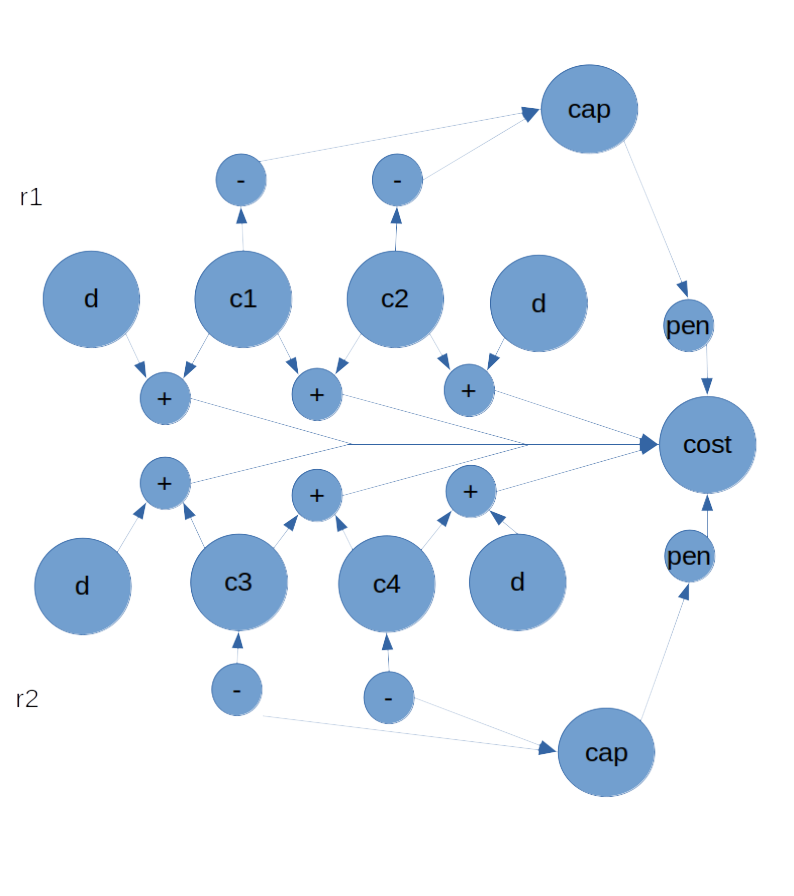
\includegraphics[width=6cm]{img/graph-1.png}
	\end{figure}
\end{frame}

\begin{frame}{Preguntas de oponencia}
	\onslide<1->\begin{figure}
		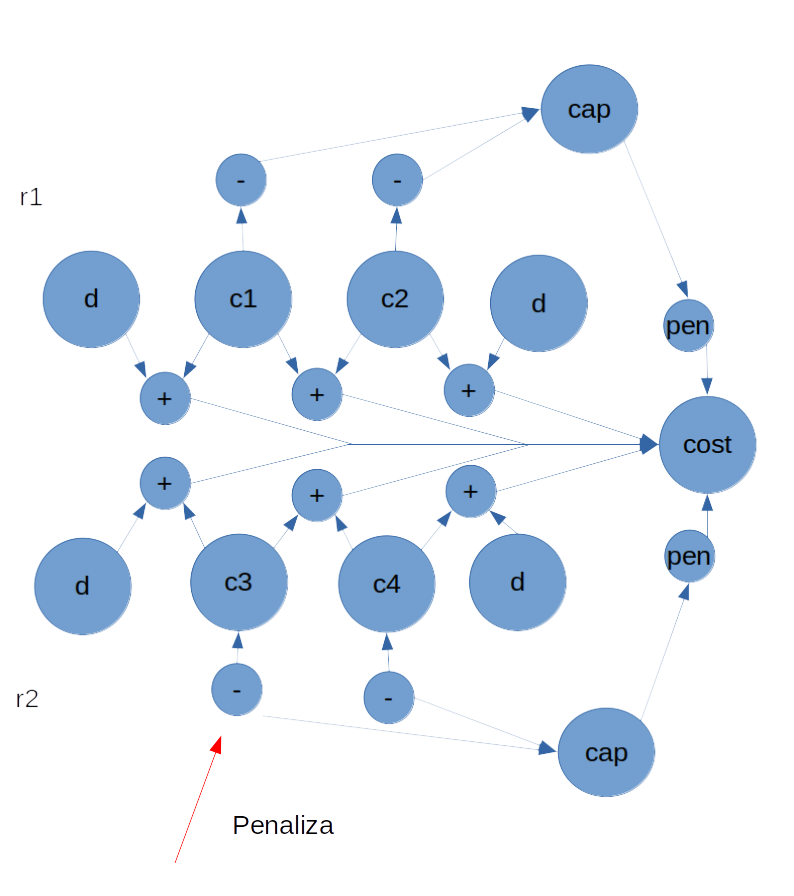
\includegraphics[width=6cm]{img/graph-2.png}
	\end{figure}
\end{frame}

\begin{frame}{Preguntas de oponencia}
	\onslide<1->\begin{figure}
		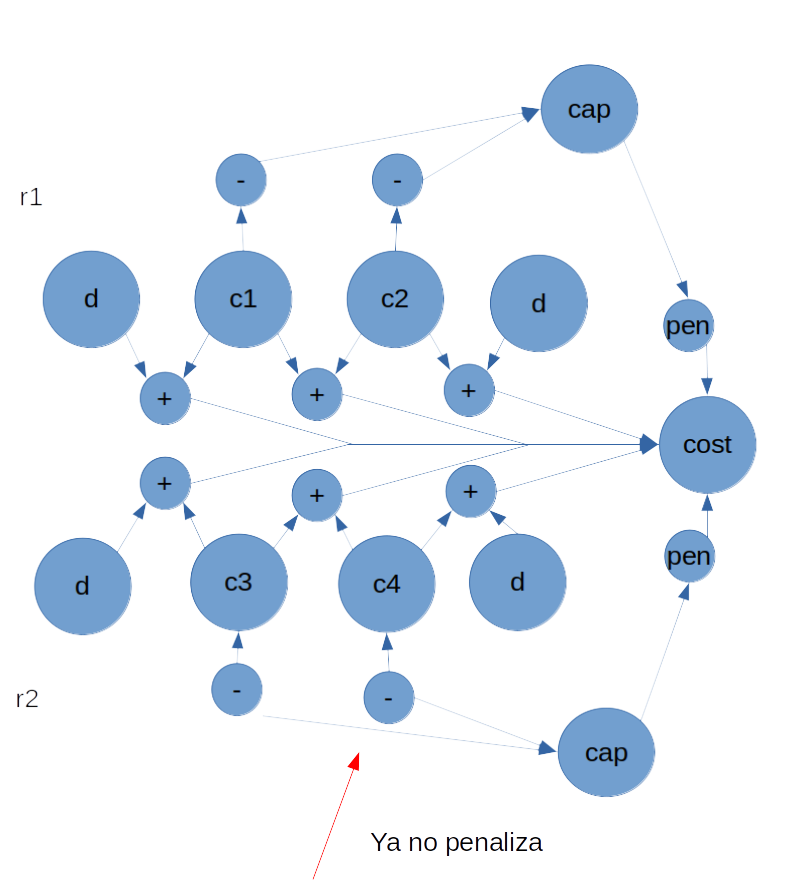
\includegraphics[width=6cm]{img/graph-3.png}
	\end{figure}
\end{frame}


\begin{frame}{Preguntas de oponencia}
	\begin{block}<1->{Pregunta 2}
		El marco de trabajo propuesto en la tesis fue desarrollado en el lenguaje de programación Common Lisp. Una razón que pudo haber motivado a tal decisión es el hecho de que algunos de los módulos utilizados en la propuesta ya estaban escritos en ese lenguaje de programación. Sin embargo, esto implica que los futuros usuarios de la propuesta deberán a su vez utilizar dicho lenguaje para describir y resolver sus problemas. Explique las ventajas que se derivan de haber seleccionado Common Lisp como lenguaje de programación, tanto para el desarrollador del marco de trabajo como para sus futuros usuarios. Considere auxiliarse de comparativas con otros lenguajes de programación para ello.
	\end{block}
	
\end{frame}

\begin{frame}{Preguntas de oponencia}
	\begin{block}<1->{Ventajas de lisp para el sistema:}
		\begin{itemize}
			\item \onslide<2->{CLOS}
		\end{itemize}
		\vspace{5.5 mm}
	\end{block}
	
\end{frame}

\begin{frame}{Preguntas de oponencia}
	\onslide<1->\begin{figure}
	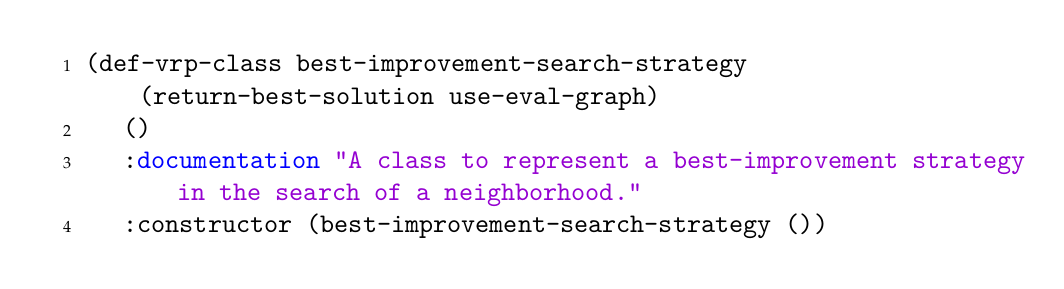
\includegraphics[width=9cm]{img/best-improvement.png}
\end{figure}

	\onslide<2->\begin{figure}
	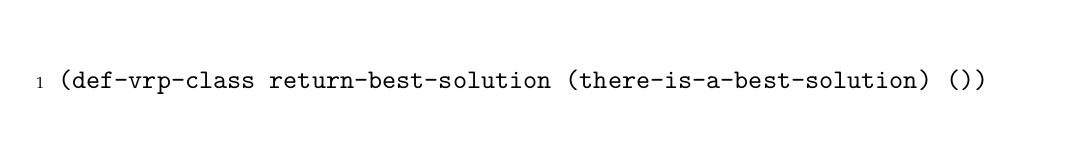
\includegraphics[width=9cm]{img/return-best.png}
\end{figure}

	\onslide<3->\begin{figure}
	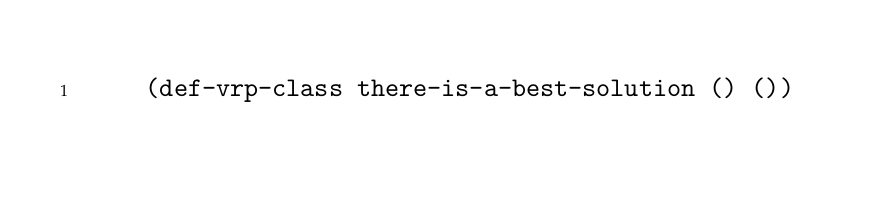
\includegraphics[width=10cm]{img/there-is-best.png}
\end{figure}
\end{frame}

\begin{frame}{Preguntas de oponencia}
	\onslide<1->\begin{figure}
		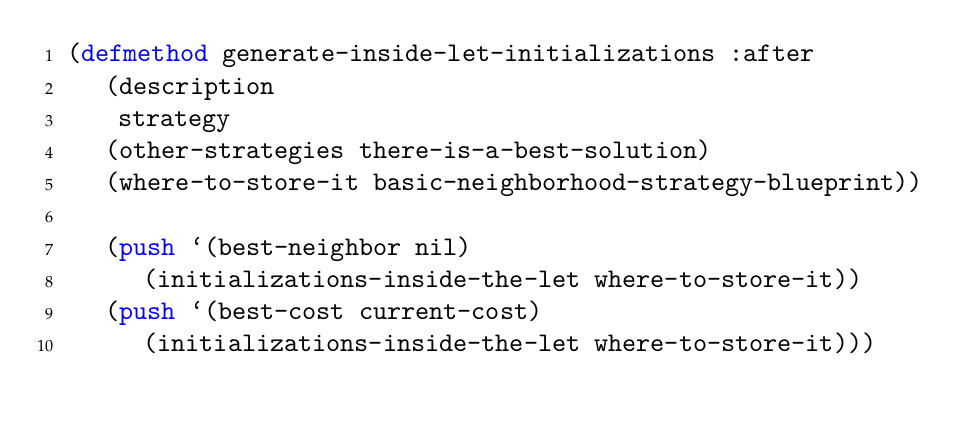
\includegraphics[width=9cm]{img/inisde-let.png}
	\end{figure}
\end{frame}

\begin{frame}{Preguntas de oponencia}
	\onslide<1->\begin{figure}
		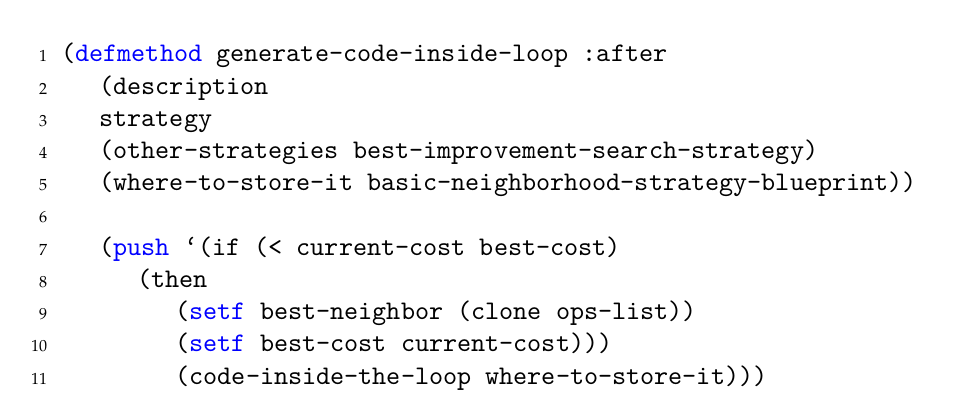
\includegraphics[width=9cm]{img/inside-loop.png}
	\end{figure}
\end{frame}

\begin{frame}{Preguntas de oponencia}
	\begin{block}<1->{Ventajas de lisp para el sistema:}
		\begin{itemize}
			\item \onslide<1->{CLOS}
			\item \onslide<2->{Generación de código fuente}
		\end{itemize}
	\end{block}
	
\end{frame}

\begin{frame}{Preguntas de oponencia}
	\begin{block}<1->{Pregunta 3}
		La propuesta de la tesis permite diseñar múltiples criterios de vecindad a partir de primitivas implementadas en el marco de trabajo. Sin embargo, como bien se discute en la tesis, es posible automatizar la generación de múltiples criterios de vecindad, lo cual eximiría al usuario final de tener que diseñar los posibles criterios de vecindad “interesantes a considerar” y, en su lugar, podría centrarse en describir el problema ¿Cuán complejo sería añadir esta característica al marco de trabajo en su versión actual? ¿Cómo lo haría?
	\end{block}
	
\end{frame}

\begin{frame}{Preguntas de oponencia}
	\begin{block}<1->{Definiendo una gramática}
		\begin{itemize}
			\item \onslide<2->{S: Elemento distinguido}
			\item \onslide<3->{S1: Selección de ruta o cliente}
			\item \onslide<4->{R1: Selección o no de una ruta}
			\item \onslide<5->{r: Selección de una ruta}			
			\item \onslide<6->{a,b,c: Selección, inserción, e intercambio de cliente}
		\end{itemize}
	\end{block}
	
\end{frame}

\begin{frame}{Preguntas de oponencia}
	\begin{block}<1->{Definiendo una gramática}
			S $\rightarrow$ r a S1 b\\
			S $\rightarrow$ r a S1 r b\\
			S $\rightarrow$ r a a S1 c\\
			S $\rightarrow$ r a r a S1 c\\
			S1 $\rightarrow$ R1 a S1 R1 b\\
			S1 $\rightarrow$ R1 a R1 a S1 c\\
			S1 $\rightarrow$ $\epsilon$\\
			R1 $\rightarrow$ r | $\epsilon$\\
	\end{block}
	
\end{frame}

\begin{frame}{Preguntas de oponencia}
	\begin{block}<1->{Generación automática de gramáticas}
		Daniela Beltrán 2019
	\end{block}

\begin{block}<1->{IVNS}
	Camila Pérez 2017
\end{block}
	
\end{frame}
